
%%%%%%%%%%%%%%%%%%%%%%% file typeinst.tex %%%%%%%%%%%%%%%%%%%%%%%%%
%
% This is the LaTeX source for the instructions to authors using
% the LaTeX document class 'llncs.cls' for contributions to
% the Lecture Notes in Computer Sciences series.
% http://www.springer.com/lncs       Springer Heidelberg 2006/05/04
%
% It may be used as a template for your own input - copy it
% to a new file with a new name and use it as the basis
% for your article.
%
% NB: the document class 'llncs' has its own and detailed documentation, see
% ftp://ftp.springer.de/data/pubftp/pub/tex/latex/llncs/latex2e/llncsdoc.pdf
%
%%%%%%%%%%%%%%%%%%%%%%%%%%%%%%%%%%%%%%%%%%%%%%%%%%%%%%%%%%%%%%%%%%%


\documentclass[runningheads,a4paper]{llncs}

\usepackage{amssymb}
\setcounter{tocdepth}{3}
\usepackage{graphicx}
\usepackage{float}
\usepackage[full]{complexity}
\usepackage{amsmath}
%\usepackage{amsfonts}
%\usepackage{amsthm}
\usepackage{subfigure}
%\usepackage{caption}
%\usepackage{subcaption}
%\usepackage{cite}
\usepackage{hyperref}
\usepackage{url}
\usepackage{clrscode4e}
\usepackage{verbatim}
\urlstyle{same}
\newcommand{\keywords}[1]{\par\addvspace\baselineskip
\noindent\keywordname\enspace\ignorespaces#1}

% Uniform numbering for previously defined theorem environments (e.g., LNCS).
\makeatletter
\let\c@lemma=\c@theorem
\let\c@corollary=\c@theorem
\let\c@fact=\c@theorem
\makeatother

% Redefinition of LNCS or SODA or Springer proof environment to put a \Box at
% the end of every proof.
\let\realendproof=\endproof
\def\endproof{\hspace*{\fill}$\Box$\realendproof}

\begin{document}

\mainmatter  % start of an individual contribution

% first the title is needed
\title{The Complexity of Determining Critical Sets}

% a short form should be given in case it is too long for the running head
\titlerunning{The Complexity of Determining Critical Sets}

% the name(s) of the author(s) follow(s) next
%
% NB: Chinese authors should write their first names(s) in front of
% their surnames. This ensures that the names appear correctly in
% the running heads and the author index.
%
\author{Fermi Ma \and Ariel Schvartzman \and Erik Waingarten}
%
\authorrunning{Fermi Ma \and Ariel Schvartzman \and Erik Waingarten}
% (feature abused for this document to repeat the title also on left hand pages)

% the affiliations are given next; don't give your e-mail address
% unless you accept that it will be published
\institute{MIT,\\
77 Mass Ave., Cambridge, MA 02139, USA, \\
\protect\url{{fermima,arielsc,eaw}@mit.edu}}

%
% NB: a more complex sample for affiliations and the mapping to the
% corresponding authors can be found in the file "llncs.dem"
% (search for the string "\mainmatter" where a contribution starts).
% "llncs.dem" accompanies the document class "llncs.cls".
%

\maketitle

\section{SAT}

In this section we show that the $\mathsf{FCP}$ version of SAT is $\mathsf{FCP}-$complete. Our proof relies on an alternative proof of the Cook-Levin theorem, described in [insert reference]. 

\begin{theorem}
$\mathsf{FCP}-SAT$ is $\mathsf{FCP}$-complete. 
\end{theorem} 

\begin{proof}

By the construction in [CL-Reference], on input $x$ we can construct in polynomial time a Boolean formula $\phi$ simulating a polynomial time Turing machine $M$. We have argued earlier that in the context of $\mathsf{FCP}$ the branching factor of a Turing machine $M$ can be reduced to $2$. Thus at each step we add variables $i_k$ which are true if and only if $M$ follows the left branch of the computation at time $k$. We then transform each claus of the form $(H_{i,k} \wedge Q_{q,k} \wedge T_{i, \sigma, k}) \rightarrow \bigvee (H_{i+d,k+1} \wedge Q_{q',k+1} \wedge T_{i,\sigma',k+1})$ into 
\[
 (H_{i,k} \wedge Q_{q,k} \wedge T_{i,\sigma, k}) \rightarrow \left(\begin{array}{c} (H_{i+d,k+1} \wedge Q_{q', k+1} \wedge T_{i,\sigma', k+1} \wedge l_k) \\ \vee \\ (H_{i+d',k+1} \wedge Q_{q'', k+1} \wedge T_{i,\sigma'', k+1} \wedge \neg l_k) \end{array}\right) 
 \]

This transformation encodes whether or not we took the left branch. We add the following clauses to obtain $\phi'$:
\[ (H_{i,k} \wedge Q_{q,k} \wedge T_{i,\sigma,k} \wedge l_k) \leftrightarrow a_{l, i, q, \sigma, k} \]
\[ (H_{i,k} \wedge Q_{q,k} \wedge T_{i,\sigma,k} \wedge \neg l_k) \leftrightarrow a_{\neg l, i, q, \sigma, k} \]

Note that there are polynomially many such clauses, which depend on the number of states of the Turing machine. We claim that $\phi$ and $\phi'$ are equivalent. Clearly, if $\phi'$ is true, then so is $\phi$ since the former contains all the clauses in the latter. If $\phi$ is satisfiable, then we know that for each time $k$, only one of each head, state, and time position variables are True, in addition, we either took the left branch, or right branch, so that gives us the value of $l_k$, so we set the corresponding $a_{l, i,q,\sigma,k}$ or $a_{\neg l, i, q, \sigma, k}$ to True and all other $a_{l, i', q', \sigma', k}$ and $a_{\neg l, i', q', \sigma', k}$ to False.
[TO FINISH]
\end{proof} 
%\begin{enumerate}
%\item We assume that we have a NTM $M$ with input $x$ running in polynomial time.
%\item We compute the Boolean formula $\phi$ corresponding to $M$ with input $x$ as in the Cook-Levin theorem.
%\item Since we assumed that $M$ has branching factor at most $2$, at each step, we add the variables $l_k$ which is True if and only if $M$ takes the left branch of the computation at time $k$.
%\item We transoform each clause $(H_{i,k} \wedge Q_{q,k} \wedge T_{i, \sigma, k}) \rightarrow \bigvee (H_{i+d,k+1} \wedge Q_{q',k+1} \wedge T_{i,\sigma',k+1})$ into 
%\[
% (H_{i,k} \wedge Q_{q,k} \wedge T_{i,\sigma, k}) \rightarrow \left(\begin{array}{c} (H_{i+d,k+1} \wedge Q_{q', k+1} \wedge T_{i,\sigma', k+1} \wedge l_k) \\ \vee \\ (H_{i+d',k+1} \wedge Q_{q'', k+1} \wedge T_{i,\sigma'', k+1} \wedge \neg l_k) \end{array}\right) \]
%Proof: Here, we are encoding in the variable $l_k$, whether we took the left branch or the right branch. Also, we are using the fact that the non-deterministic transition contains only two possible branches.
%\item We add the following clauses to obtain $\phi'$:
%\[ (H_{i,k} \wedge Q_{q,k} \wedge T_{i,\sigma,k} \wedge l_k) \leftrightarrow a_{l, i, q, \sigma, k} \]
%\[ (H_{i,k} \wedge Q_{q,k} \wedge T_{i,\sigma,k} \wedge \neg l_k) \leftrightarrow a_{\neg l, i, q, \sigma, k} \]
%Proof: We can do this without increasing $\phi$ too much since we have $O(p(|x|)^2)$ clauses.
%\item $\phi'$ is satisfiable if and only if $\phi$ is satisfiable. \\
%Proof: We know whenever $\phi'$ is satisfiable, $\phi$ is satisfiable since it contains more clause requirements. Now if $\phi$ is satisfiable, then we know that for each time $k$, only one of each head, state, and time position variables are True, in addition, we either took the left branch, or right branch, so that gives us the value of $l_k$, so we set the corresponding $a_{l, i,q,\sigma,k}$ or $a_{\neg l, i, q, \sigma, k}$ to True and all other $a_{l, i', q', \sigma', k}$ and $a_{\neg l, i', q', \sigma', k}$ to False.
%\item Let $P$ be the smallest partial assignment of the variables in $\phi'$ such that $\phi'$ is uniquely satisfiable after the assignment.
%\item In order to simplify notation, we use $l'$ be the literal $l$ or $\neg l$.
%\item Suppose some $a_{l', i, q, \sigma, k}$ in $P$ is assigned to False, then we can replace it with some other $a_{l'', i', q', \sigma', k}$ which is assigned to True. \\
%Proof: In the unique solution, there is some $a_{l', i', q', \sigma', k}$ which is True. We also know that $a_{l'', i',q',\sigma',k} \rightarrow \neg a_{l',i, q, \sigma, k}$ since there can only be one state variable, one head position variable, and one tape cell variable for that head position be True at that time. 
%\item We can find this is alternate $a_{l'', i', q', \sigma', k}$ in polynomial time.\\
%Proof: There are polynomially many $a_{l'', i',q',\sigma',k}$ so we can write the formula $\phi'$ which remains after all the $P - \{a_{l', i, q, \sigma, k}\}$ are assigned. Furthermore, we assign $a_{l'', i', q',\sigma', k}$ and check whether the smallest partial assignment of this formula is empty (i.e. there exists a unique solution).
%\item Likewise, if there is any other type of variable in $P$ which is assigned to False, we can replace it with a True variable.\\
%Proof: the same procedure works as in $6$ and $7$ work.
%\item If some variable in $P$ is not a variable of type $a$, then we can replace it by a variable of type $a$.\\
%Proof: Existance holds since at that step, there is an action taken by NTM $M$, and we can find it by the same procedure as in $7$. 
%\item So we can find a smallest partial assignment $P$ made up of all variables of the form 
%\[ a_{l', i,q,\sigma, k} \]
%Proof: follows from $7$ and $9$.
%\item The variables $a_{l', i,q,\sigma, k}$ being True, indicate whether at a given time, $M$ took a left branch or a right branch.\\
%Proof: In fact, we have complete information of the transition NTM $M$ made at the $k$th step. If $l' = l$, then we took a left branch, if $l' = \neg l$, then we took a right branch.
%\item If the partial assignment has a unique satisfying assignment, then the mNTM $M$ has a unique accepting branch. \\
%Proof: This follows from $14$ and the fact that each assignment of the variables corresponds bijectively with a branch of the computation of $M$. 
%\item The smallest partial assignment with a unique satisfying assignment is the same size as the smallest partial certificate with a unique accepting branch.\\
%Proof: For each variable, we have one indication of a branch, and for each transition made by an accepting branch, we have a variable in the partial certificate. 
%\end{enumerate}
%
%\begin{itemize}
%\item $f$ is the Cook-Levin construction, and add variables $a_{l, q, i, j, k}$ to indicate whether took left branch at time $k$ from state $q$ and wrote at $i$ character $j$. 
%\item $C_B'$ is the set of clues involving only true values of $a_{l,q,i,j,k}$ and full solutions.
%\item $M$ takes variables which are false and finds the ones that are true. This is done in polytime since a variable being true, implies one being false. We know that one must be true, so we can look for it. $M$ sets $a_{l,q,i,j,k}$ while removing other variables.
%\item $g$ sends $a_{l,q,i,j,k}$ which is true into took $l$ branch at time $k$.
%\end{itemize}
%
%Note that algorithm $M$ takes minimal to minimal since any false variable can be replaced, and any non-$a$ variable can be replaced with an $a$ variable which implies it. 
%
%$g$is surjective, since for each right-branch, left-branch, there exists a set of $a$'s set to True. $g$ is bijective on the solutions since Cook-Levin is parsimonious. If $c_1 \subset c_2$, then $g(c_1) \subset g(c_2)$ since $g$ maps each element for $c$.

\section{3SAT}

In this section we show that the $\mathsf{FCP}$ version of 3-SAT is also $\mathsf{FCP}-$complete. 

\begin{theorem}
$\mathsf{FCP}-3SAT$ is $\mathsf{FCP}$-complete. 
\end{theorem} 

\begin{proof}
We reduce from $\mathsf{FCP}-3SAT$. We will define a recursive mapping $f$ from instances of SAT to those of 3-SAT. Suppose we are given a SAT formula $\phi$ with clauses $C_i$. If $|C_i| \leq 3$, then we preserve the clause. Otherwise, if $C_i$ has $k$ variables $x_1,...,x_k$ we replace the original clause with 
\[ 
(x_1 \vee x_2 \vee z_2) \wedge (\overline{z_2} \vee \overline{x_2}) \wedge (z_2 \vee x_2) \wedge f(\overline{z_2}, x_3, ..., x_k) 
\]

where the last term indicates we keep recursing until each clause has at most $3$ variables. Note that on each step we reduce the number of variables in the longest clause by at least $1$, so after $O(n)$ steps (per clause) we will have a valid 3-SAT instance at the cost of adding variables and small clauses. It is not hard to see that the original clause and it's mapped version agree on solutions. Notice that by construction $x_i \iff \overline{z_i}$. 

Suppose we are given a clue set $C_B$ for 3-SAT. The mapping $g$ from $C_B$ can return a set of the same size that is valid for SAT by assigning $x_i = \overline{z_i}$ if given $z_i$ or simply returning the same $x_i$. This implies that if we are given a minimal clue set for 3SAT we can return a minimal clue set for SAT as well (because whenever we add a clue we remove another one). It is clear that $g$ maps subsets since it is bijective and maps individual elements. 

\end{proof}

\subsection{NAE-3SAT}

\begin{theorem}
$\mathsf{FCP}-NAE-3SAT$ is $\mathsf{FCP}$-complete. 
\end{theorem} 

\begin{proof}
We claim that the reduction for 3SAT is sufficient to show this. Note that the 3SAT instance created will never have all the elements in a clause set to true, therefore being a valid NAE-3SAT instance. 
\end{proof}

%\subsection{1-in-3 SAT}
%
%
%\begin{theorem}
%$\mathsf{FCP}-1-in-3SAT$ is $\mathsf{FCP}$-complete. 
%\end{theorem} 
%
%\begin{proof}
%We claim that the reduction for 3SAT is also sufficient to show this. Consider the following change in the mapping presented. Rewrite the clauses of the form  $(x_1 \vee x_2 \vee z_2)$ to 
%
%$$(x_1 \vee z_1) \wedge (\overline{z_1} \vee \overline{x_1}) \wedge (\overline{z_1} \vee x_2 \vee z_2).$$
%
%Then no clause will ever have more than one variable set to true, creating a valid 1-in-3SAT instance.  
%\end{proof}

\section{Triangle Partition}
[TO CHECK] 
In the triangle partition problem we are given a graph $G = (V,E)$ and want to find a partition of the $V$ into vertex-disjoint triangles. Holyer  \cite{holyer1981np} showed this problem is $\NP$-complete. We claim that it is also $\mathsf{FCP}$-complete and refer to elements of his proof. 

\begin{theorem}
$\mathsf{FCP}$ Triangle Partition is $\mathsf{FCP}$-complete.
\end{theorem}

\begin{proof}
We refer the reader to \cite{holyer1981np}, \cite{colbourn1984complexity} for questions about notation. We will show a special subset clue reduction from $\mathsf{FCP}$-SAT. 

We define $f$ to map instances of SAT to Triangle Partition as in \cite{holyer1981np}. For a given instance of Triangle Partition with clues, we let its special clue set $C_B'$ be the clues with at most one particular triangle per $H_{3,p}$ graph. We map the first true literal of each clause to an $F$-partition. The algorithm $M$ then translates toe triangles to these particular triangles and moves the triangles in clauses so that the first true literal is in $F$-partition. The mapping $g$ then simply projects variables, making it a surjective function that also preserves subsets since it maps elements to elements. It is also bijective on solutions since we made $C_B'$ assign clauses in ambiguous cases.   
\end{proof}

\section{Latin Squares}

In Latin Squares we are given a $n \times n$ grid, some of whose entries have been filled in with numbers from $1$ to $n$. The goal of the game is to fill the rest of the grid with numbers from $1$ to $n$ while enforcing that no row or column repeats a number. It is known that such problem is $\NP$-complete and it can be shown that its $\mathsf{FCP}$ version is $\mathsf{FCP}-complete$. 

\begin{theorem}
$\mathsf{FCP}$ Latin Squares is $\mathsf{FCP}$-complete.
\end{theorem}

\begin{proof}
We do this via reduction from $\mathsf{FCP}$ TrianglePartition. Throughout this proof we will be using constructions and results from  \cite{colbourn1984complexity}.

Given a tripartite graph $G$, we first check whether or not it is uniform. If it is not uniform, then there does not exist a triangle partition. If it is uniform, we can write down a Latin framework $LF(G;2n,2n,2n)$ in polynomial time  \cite{colbourn1984complexity}. This Latin framework is constructed so that $G$ is the defect graph of $LF(G;2n,2n,2n)$. We then simply map via $f$ instances of defect graphs $G$ to partial Latin Squares. The Latin Squares clues are mapped to triangles with vertices on different parts of the partition. Each clue is mapped, by construction, bijectively to a triangle (since the triangle takes into account the row, column and number of the clue). As Colbourn shows, there is a triangle partition of $G$ if and only if we can complete the partial Latin Square $LF(G;2n,2n,2n)$. This implies that the triangle partitions of a defect graph $G$ are in one to one correspondence with the solutions to its Latin Square. This completes the proof. 

\end{proof}

\section{Sudoku}

In Sudoku, or Number Place, we are given a $n^2 \times n^2$ grid consisting of $n^2$ $n \times n$ bolded blocks, some of whose entries have been filled in with number from $1$ to $n^2$. The goal of the game is to fill in the rest of the grid with numbers from $1$ to $n^2$ while enforcing that no row, column or bolded square repeats a numbers. We will show this problem is FCP-Complete by providing a reduction from FCP-Latin Squares. 

Before showing the main result of this section, we will exhibit a particular way to fill a Sudoku puzzle. Next, we will show how this particular solution can be used to explicitly map instances of Sudoku to instances of Latin Squares. For simplicity, throughout this argument we will be using numbers in the range $0$ through $n^2 - 1$. We will refer to the entry on the $i$-th row and $j$-th column of a Number Place puzzle as $S(i,j)$.

\begin{proposition}
Let $S_0$ be defined as
$$S_0 (i,j) = ((i \mod n) n + \lfloor i/n \rfloor + j) \mod n^2. $$
Then $S_0$ represents a solution to an order $n$ Number Place.
\end{proposition}

\begin{proof} 
Omitted. See [Yato and Seta] 
\end{proof}

\begin{lemma}
Let $S$ be a Sudoku instance of order $n$ such that
\begin{displaymath}
S(i,j) = \left\{
\begin{array}{lr}
\perp & : (i,j) \in B\\
S_0 (i,j) & : \text{otherwise}
\end{array}
\right.
\end{displaymath}

where $B = \{ (i,j) | i < n \text{ and } (j \equiv 0) \mod n \}$. Then a square $S'$ obtained by filling in the blanks of $S$ is a solution to $S$ if and only if

\begin{itemize}
\item For any $(i,j) \in B$, $S'(i,j) \equiv 0 \mod n$
\item A square $L$ defined by $L(i, j/n) = S'(i,j)/n$ for all $(i, j) \in B$ is a Latin Square.
\end{itemize}

\end{lemma}

\begin{proof} 
Omitted. See [Yato and Seta] 
\end{proof}

\begin{lemma} 
FCP-Sudoku is FCP-Complete
\end{lemma}

\begin{proof} 
We will show a reduction via FCP-Latin Squares. We use the injective map from instances of Latin Square to instances of Sudoku described above. Let $C_B$ be the set of set of clues of Sudoku. Then we can let $g(C_B)=C_B$, mapping the clues from $S(i,j)$ (where the $(i,j) \in B$) to $L(i, j/n)$.This mapping is surjective, bijective on solutions by the lemma above and preserves subsets. Therefore, FCP-Sudoku is FCP-Complete. 
\end{proof}

\begin{figure}[H]
\begin{minipage}{0.45\textwidth}
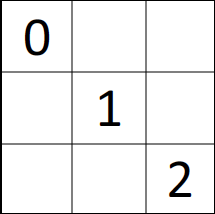
\includegraphics[scale=0.25]{sudoku-3.png}
\label{fig:partialNP}
\end{minipage}
\hfill
\begin{minipage}{0.45\textwidth}
\centering
\label{fig:partialLS}
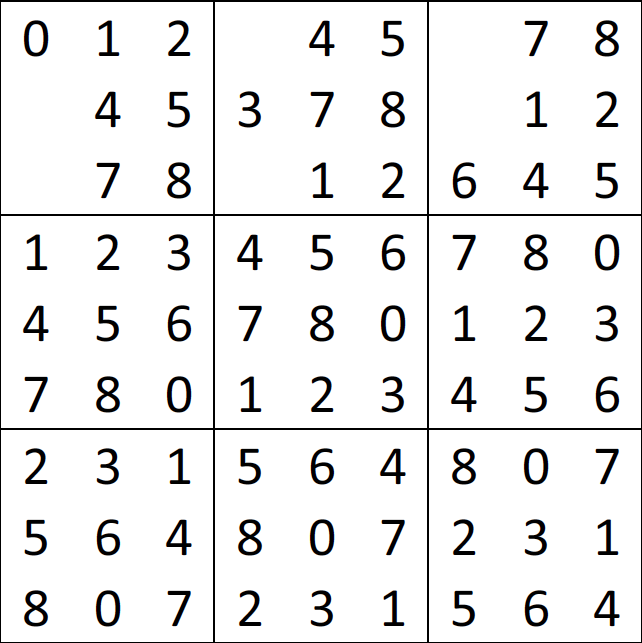
\includegraphics[scale=0.25]{sudoku-1.png}
\end{minipage}
\caption{Example of a mapping between instances of Latin Squares and Sudoku.}
\end{figure}

%\section{3-colorability}
%
%We have a reduction from 3SAT. 
%\begin{figure}
%\centering
%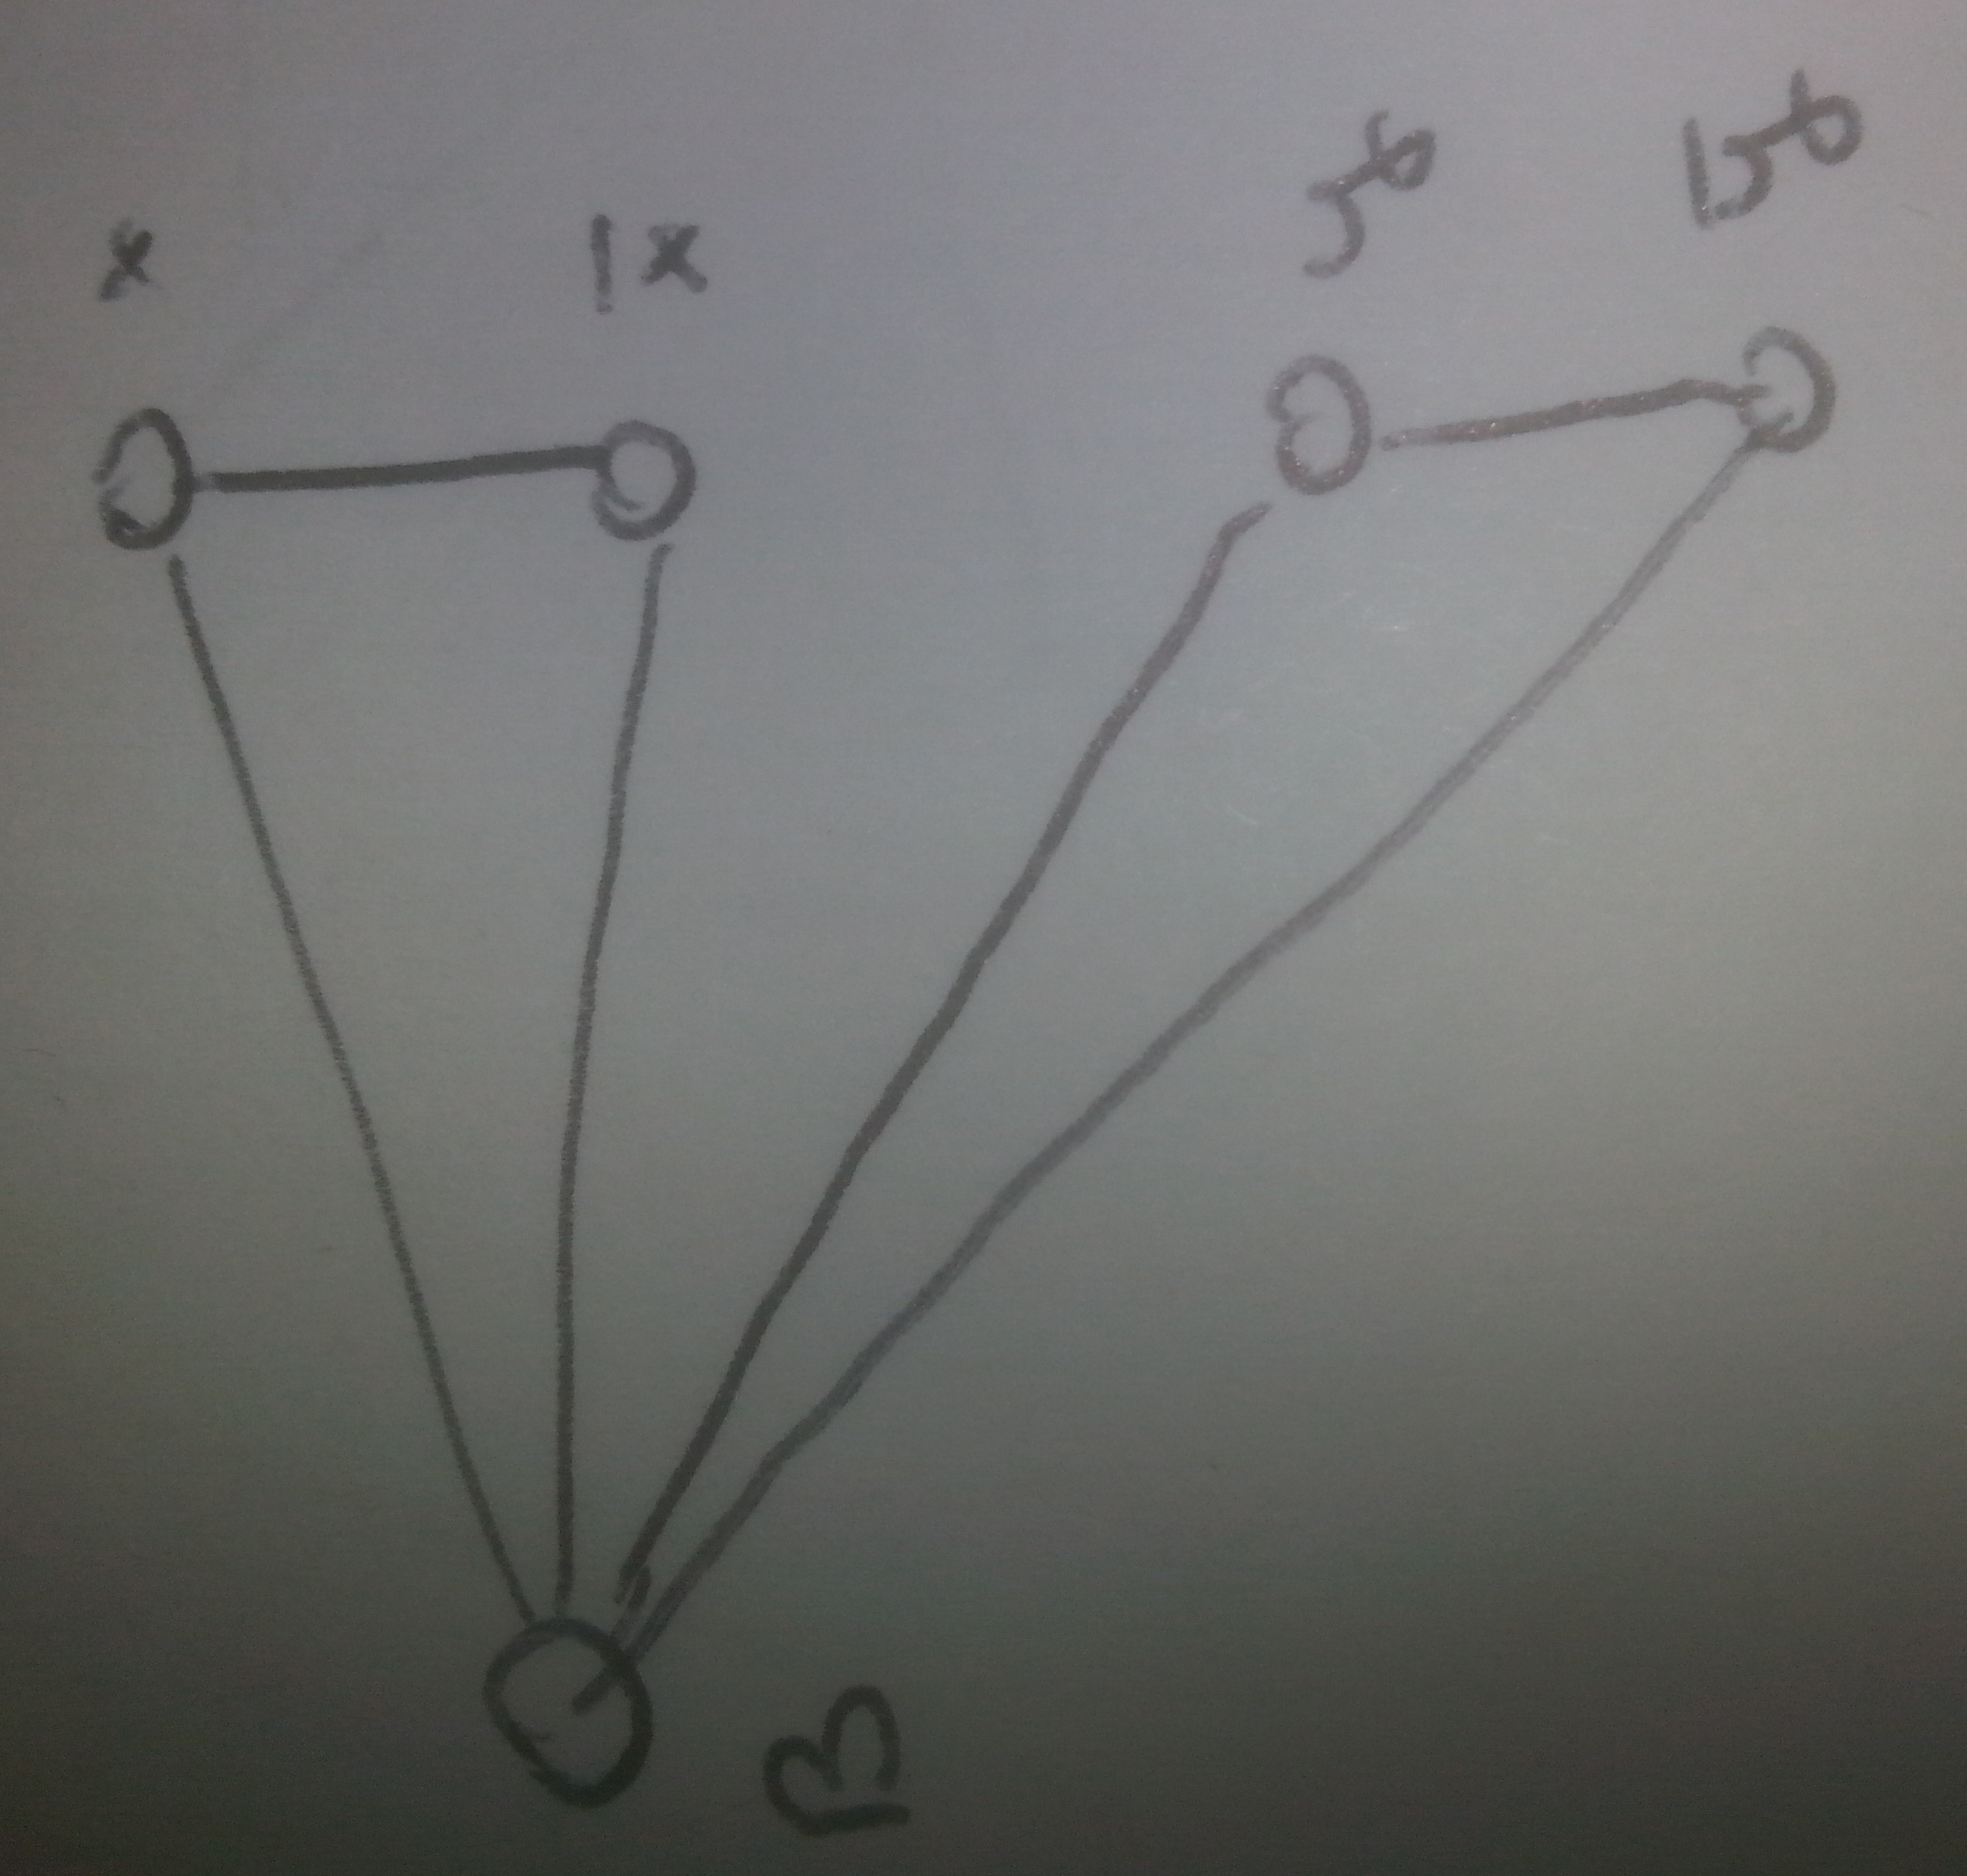
\includegraphics[width=0.3\linewidth, angle=-90]{3colorable-var.jpg}
%\caption{variable gadget}
%\end{figure}
%
%\begin{figure}
%\centering
%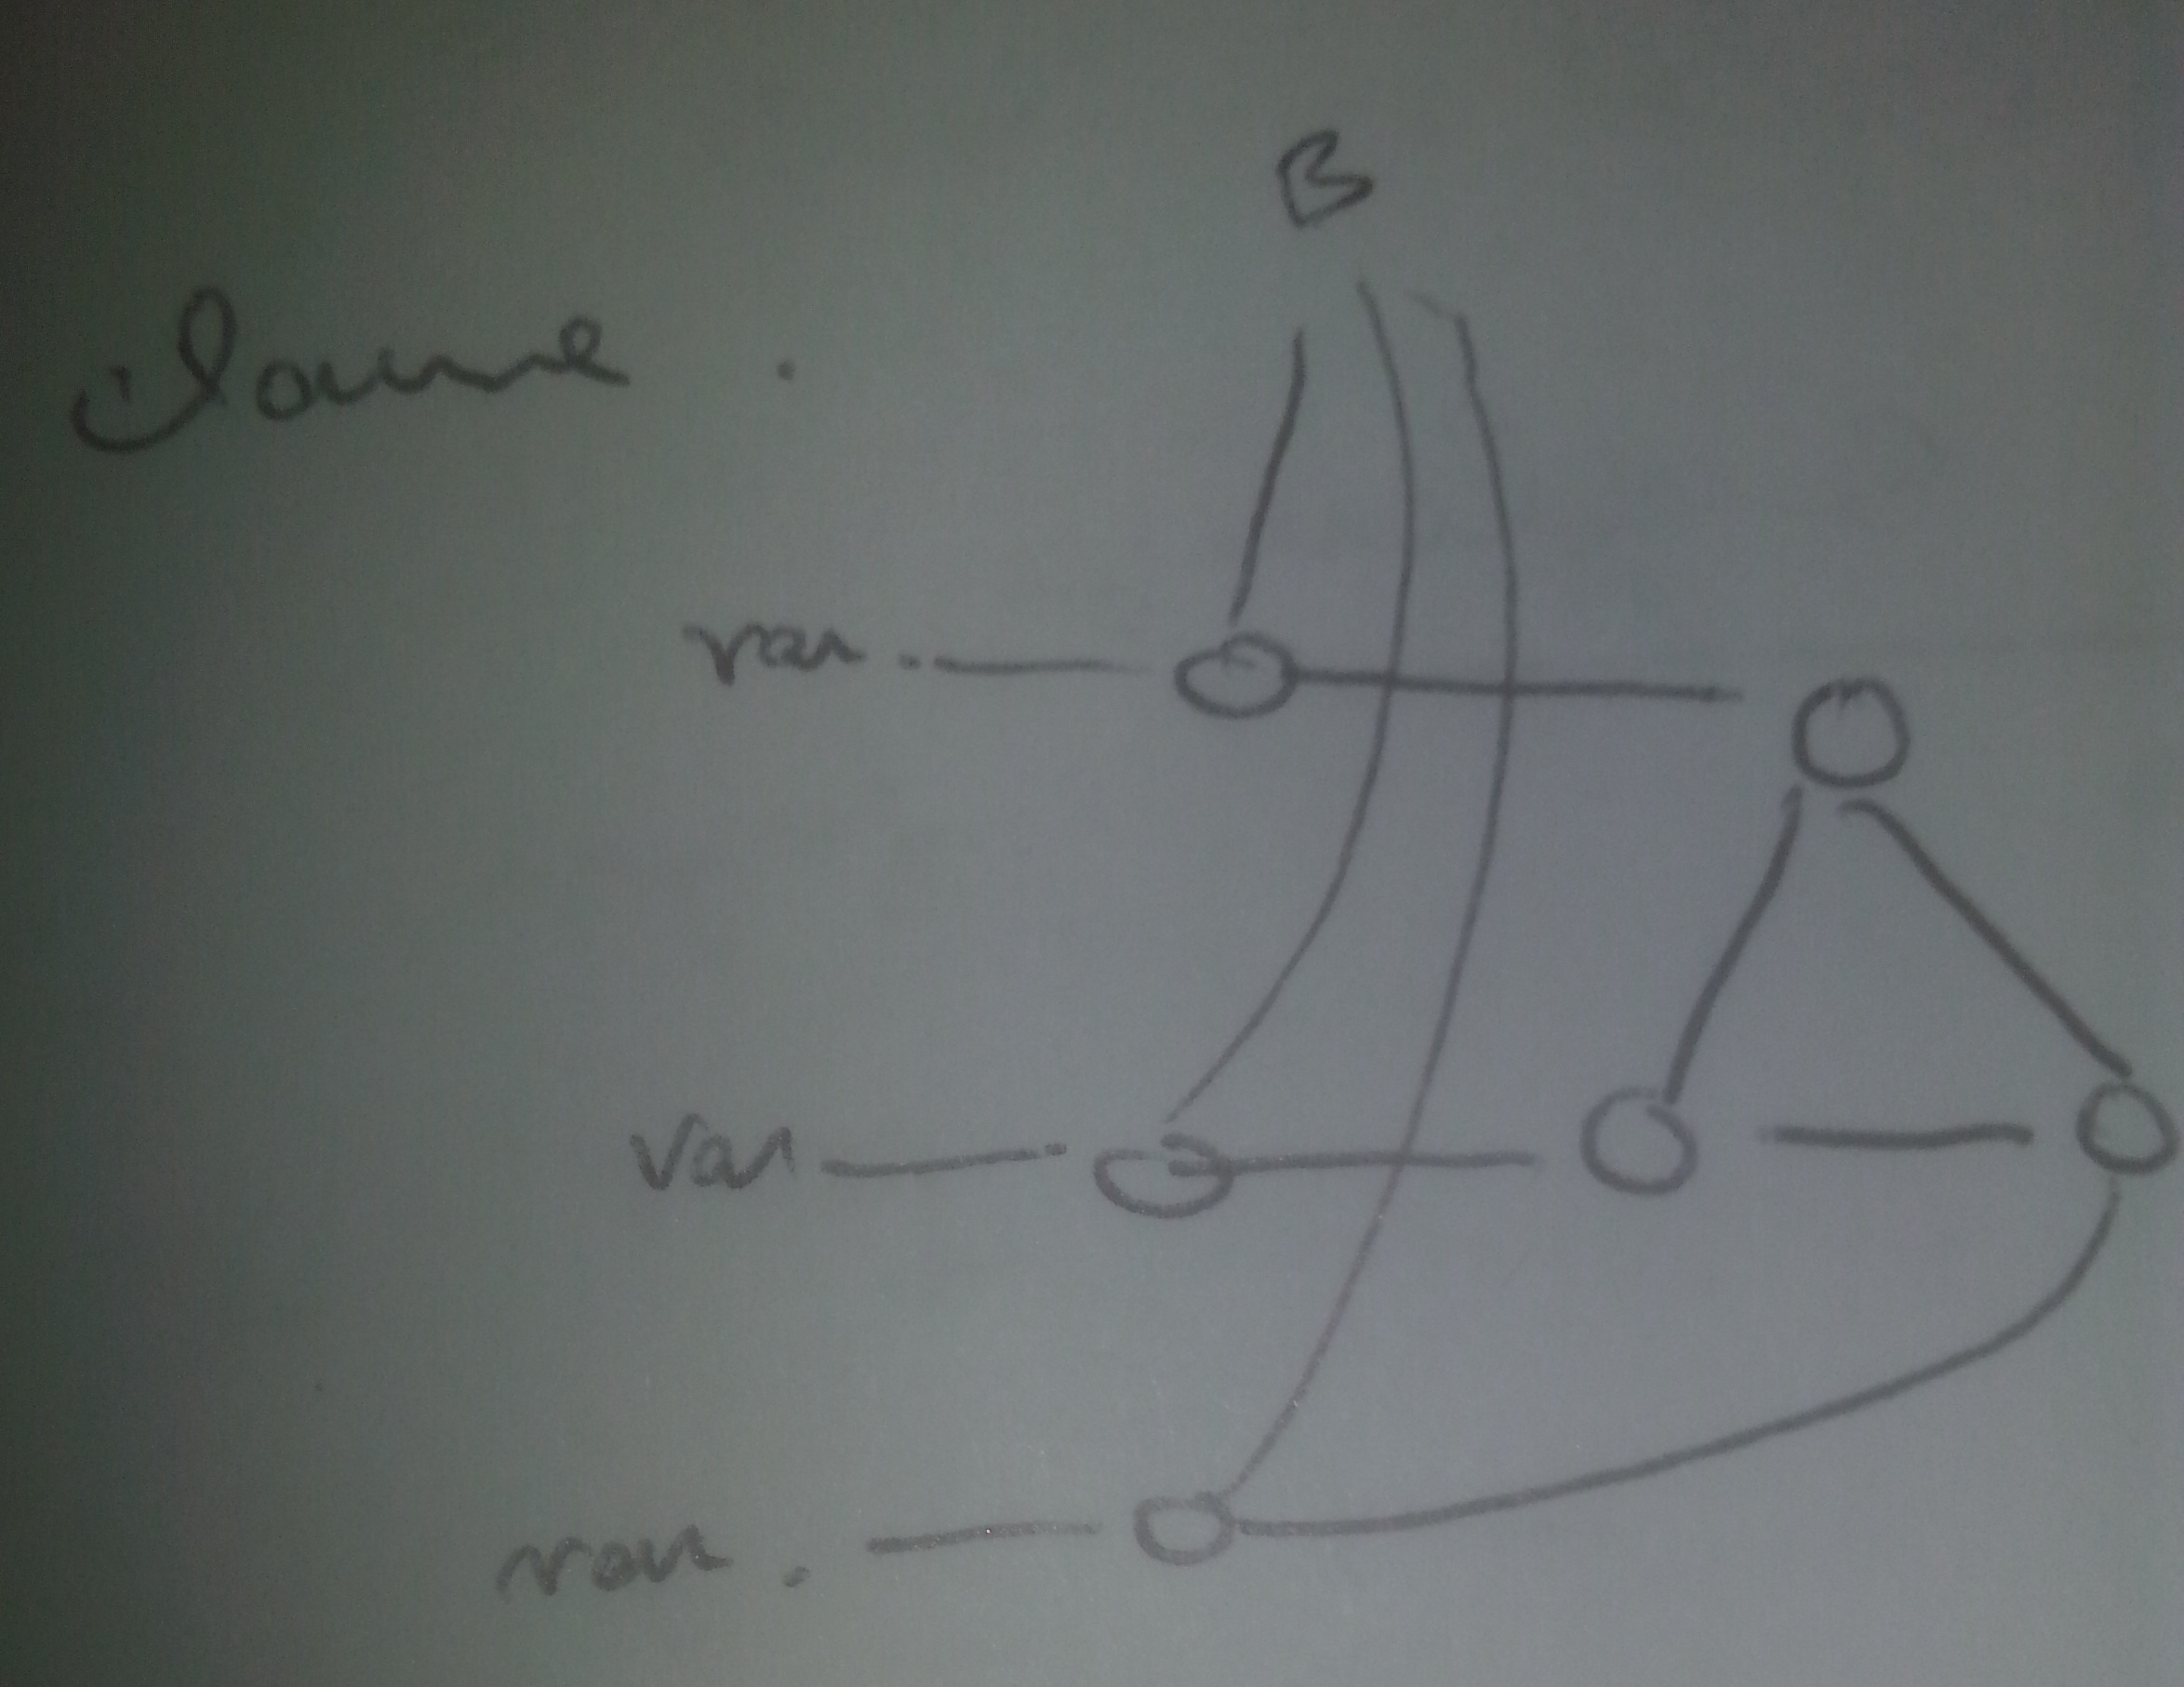
\includegraphics[width=0.3\linewidth]{3colorable-clause.jpg}
%\caption{clause gadget}
%\end{figure}
%
%Now we can do a similar thing as in triangle partition and make the F colors in the clause be the first ones written out. We also note that this throws away information, so it makes sense that it is still $\mathsf{FCP}$-hard. Furthermore, if the formula is planar, then the graph can be turned planar, with the following transformation, where also we keep alternating up between $x, \overline{x}, x, \overline{x}, ... $ so that each appearence connects to one, and since these are connected in a path (also all to $B$), they will have the same color.
%
%\begin{figure}
%\centering
%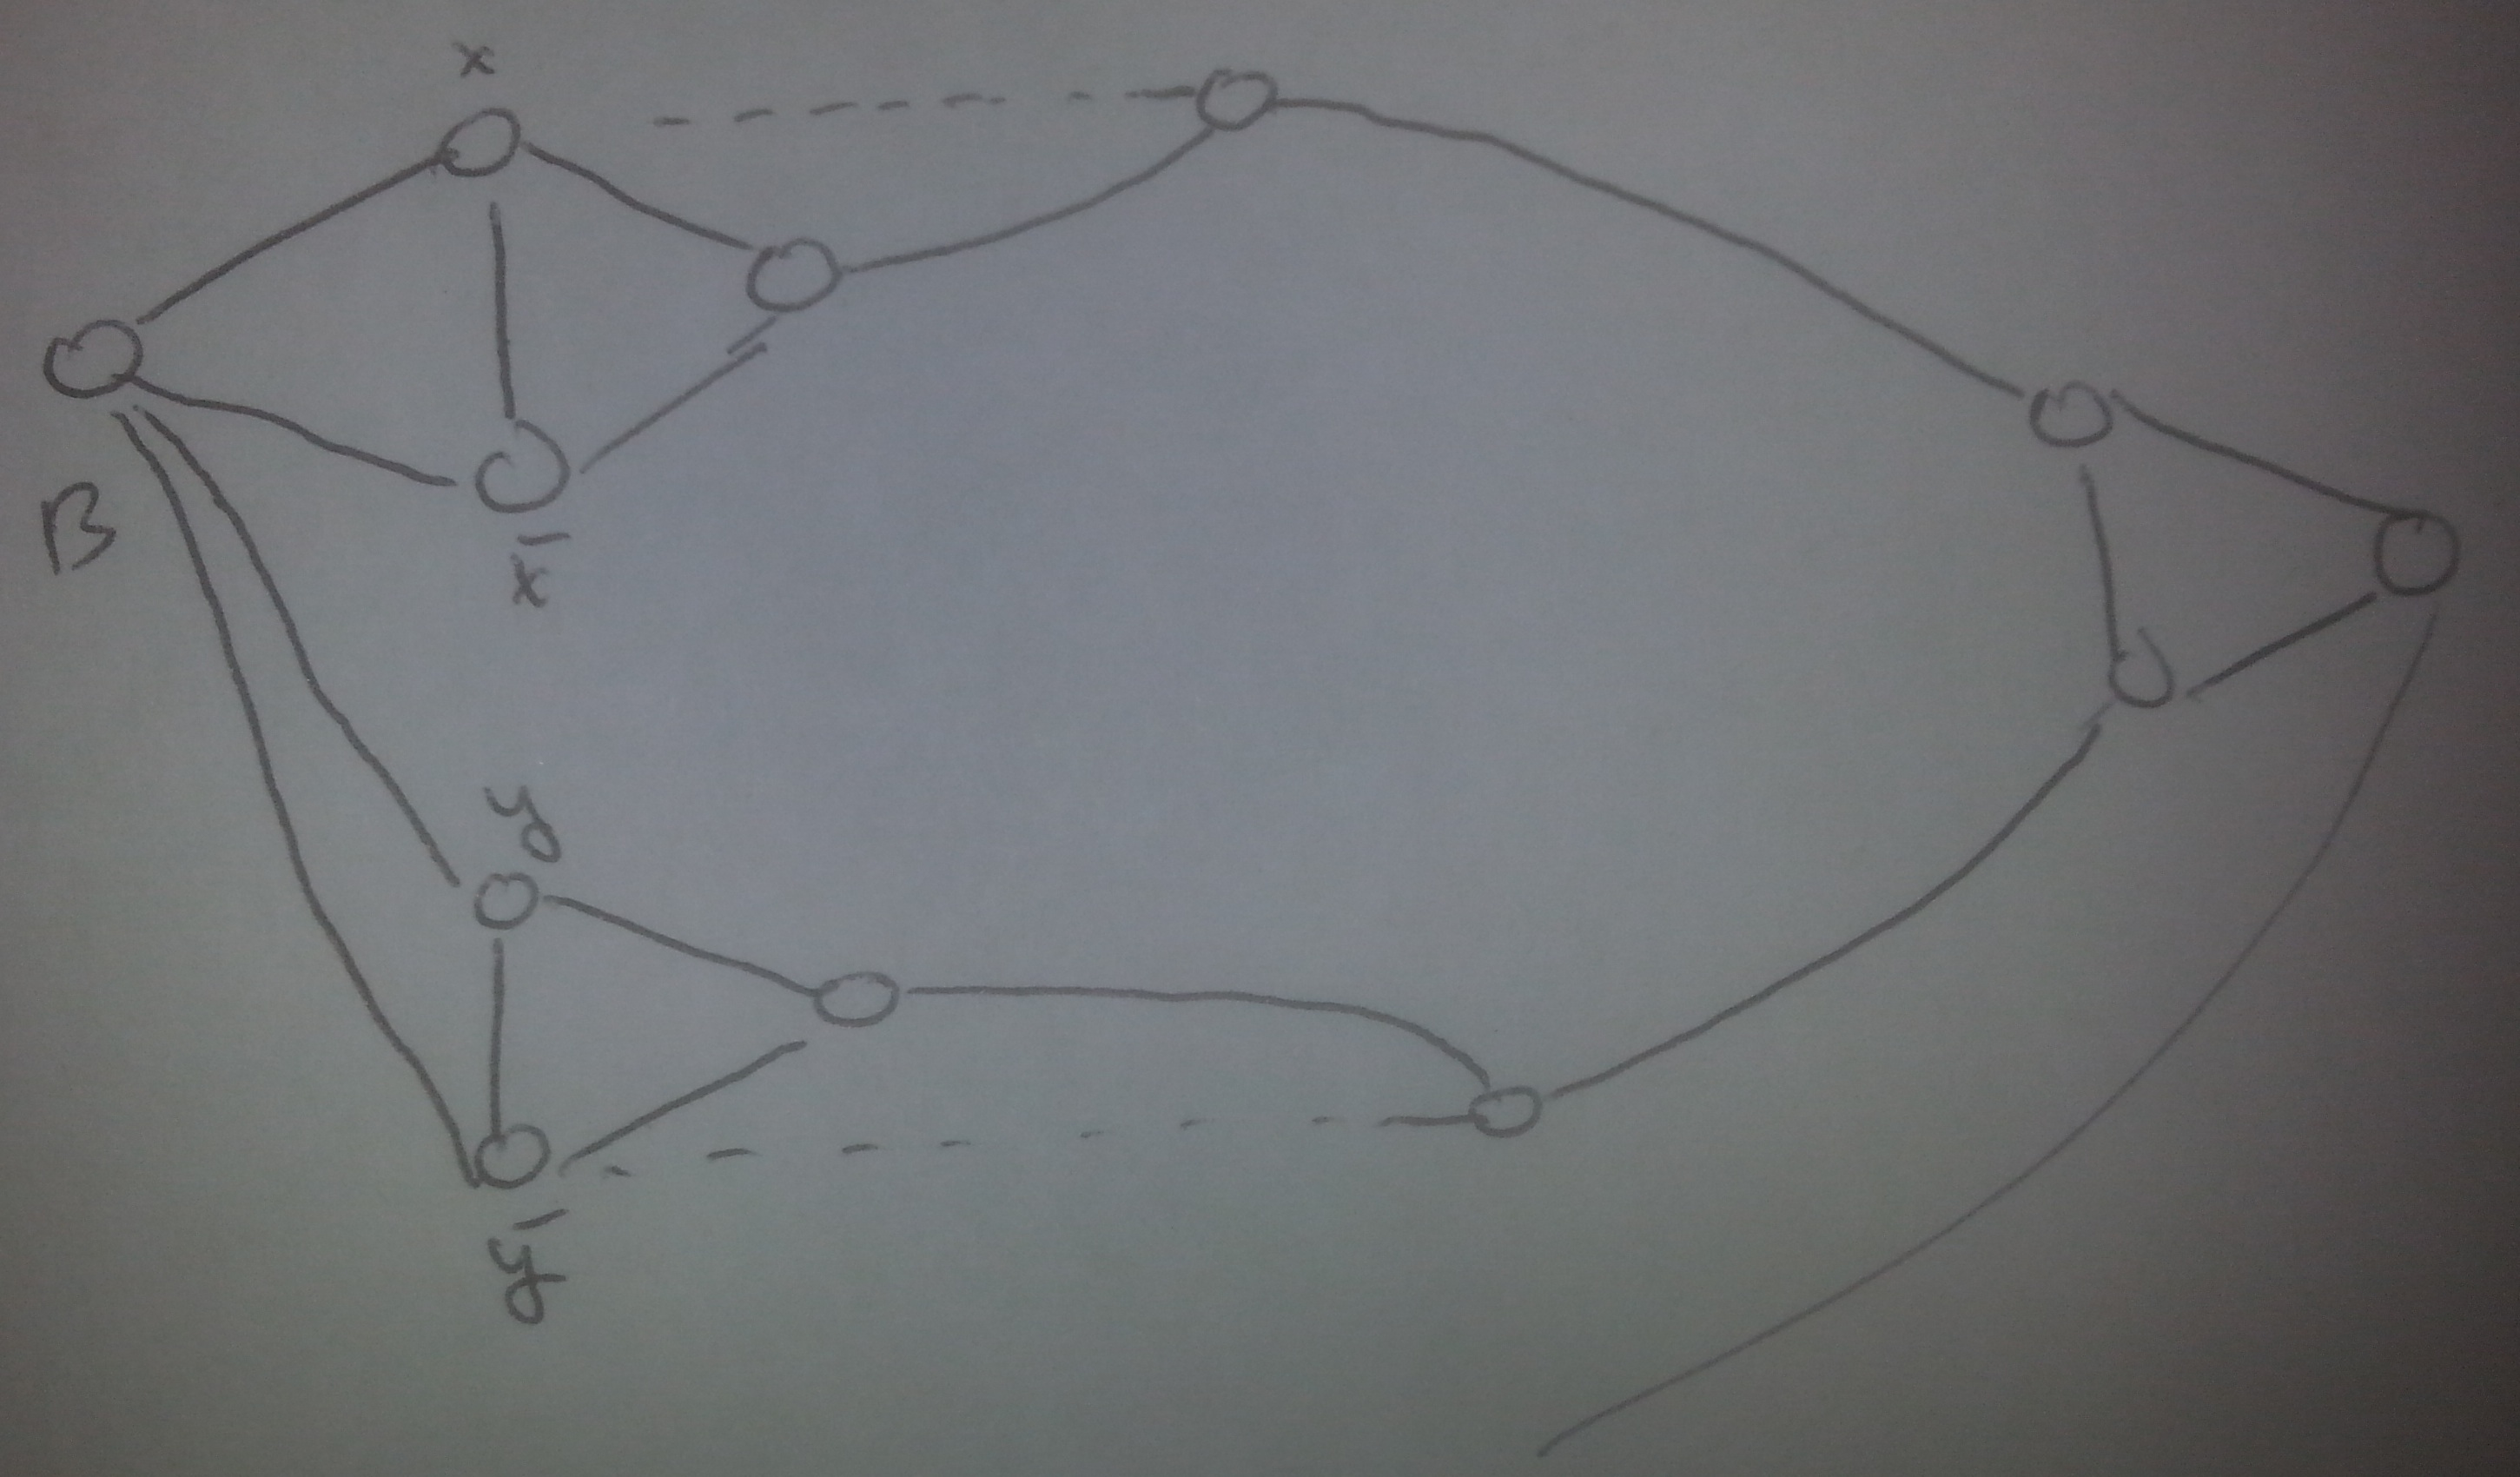
\includegraphics[width=0.4\linewidth]{3colorable-planar.jpg}
%\caption{making the reduction planar}
%\end{figure}
%
%\section{Bag - Corral}
%
%If we assume that planar 3-coloring is $\mathsf{FCP}$-hard, then Corral is $\mathsf{FCP}$-hard. The clues here are lists of edges that are included in the graph. We can use the reduction from \url{http://www2.stetson.edu/~efriedma/papers/corral/corral.html} and note that since for each wire there are three possible fillings, the clues can be moved, and each implies the next, until we get to a turn (in particular, this corresponds to the edges that border the colors, but not true ones. Therefore, we can move the final solution to the values of the vertices. And so we can  three-color the graph, since in a vertex, we know how to color them since we know which edge starts the signal.
%
%\section{Indepedent set}
%
%Trivial. Using reduction from \url{https://www.cs.cmu.edu/~ckingsf/bioinfo-lectures/sat.pdf}

\end{document}
